% SEGMENT OLP-0018-S01
% Part: sets-functions-relations
% Chapter: relations
% Section: trees

\documentclass[../../../include/open-logic-section]{subfiles}

\begin{document}

\olfileid{sfr}{rel}{tre}
\olsection{மரவுருக்கள்}

தருக்கவியலின் அனைத்துப் பகுதிகளிலும் முக்கியப் பங்காற்றும் ஒரு குறிப்பிட்ட
வகைப் பகுதி வரிசை \emph{மரவுரு} ஆகும். தருக்கவியலின் தொடக்கநிலைப்
பகுதிகளிலேயே முடிவுறு மரவுருக்கள் வருகின்றன: எடுத்துக்காட்டாக,
!!{formula}s சிதைக்கப்பட்டு ஓர் இலக்கண அமைப்பு மரவுருவாக
அமைவதைக் கொண்டு அவற்றைப் புரிந்துகொள்ளலாம். அதேபோல, பல
!!{derivation} அமைப்புகளில் !!{derivation}s முடிவுறு மரவுருக்களின்
வடிவத்தைக் கொள்கின்றன.
%
கூற்றுத் தருக்கவியல், முதல்நிலைத் தருக்கவியல் ஆகியவற்றின் நிறைவுத்
தேற்றங்களின் நிறுவலிலேயே முடிவிலி மரவுருக்கள் தோன்றுகின்றன;
கணிதத் தருக்கவியல் முழுவதும் அவை பயன்படுகின்றன.

% SEGMENT OLP-0018-S02
கணக்கோட்பாட்டில் மரவுரு என்ற கருத்துக்கும், கோட்டுருக் கோட்பாட்டில் மரவுரு
என்ற கருத்துக்கும் நெருங்கிய தொடர்பு உள்ளது. ஒரு (முடிவுறு) மரவுருவின்
படம் இங்கே தரப்படுகிறது:

\begin{center}
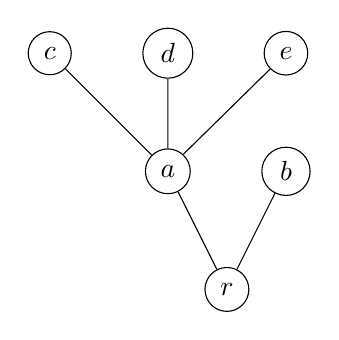
\begin{tikzpicture}[nodes={draw, circle}, -]
\node{$r$} [grow'=up]
    child { node {$a$}
        child { node {$c$} }
        child { node {$d$} }
        child { node {$e$} }
    }
    child { node {$b$} };
\end{tikzpicture}
\end{center}

மிகவும் கீழே உள்ள கணு $r$ தான் வேர். $r$ தவிர ஒவ்வொரு கணுவுக்கும்,
அதற்கு உடனே கீழே, சரியாக ஒரு பெற்றோர் கணு உள்ளது.
விளிம்புகளைப் பின்பற்றி மேல்நோக்கிச் செல்வதன் மூலம் $x$ இலிருந்து $y$ ஐ
அடைய முடியும்போது, கணு $x$ க்கும் கணு $y$ க்கும் இடையிலுள்ள தொடர்பை,
$x$ என்பது $y$ இன் \emph{முன்னோர்} என்பதாகக் கருதலாம்.

% SEGMENT OLP-0018-S03
ஒரு மரவுருவில் முன்னோர் தொடர்பு ஒரு கண்டிப்பான பகுதி வரிசையாகும்.
இது கணக்கோட்பாட்டு வரையறைக்குத் தூண்டுதலாக அமைகிறது. அந்த வரையறையைக்
கூற இரு கருத்துகள் தேவை. $\le$ மூலம் பகுதி வரிசைப்படுத்தப்பட்டுள்ள
$A$ என்ற கணத்தில் ஒரு \emph{மீச்சிறு உறுப்பு} என்பது, எல்லா
$y \in A$ க்கும் $x \le y$ என அமையும் !!a{element} $x \in A$ ஆகும்.
ஒரு கணத்தின் ஒவ்வொரு வெற்றற்ற உட்கணத்திற்கும் ஒரு மீச்சிறு உறுப்பு
இருந்தால், அக்கணம் $\le$ மூலம் \emph{நன்கு வரிசைப்படுத்தப்பட்டுள்ளது}
என்கிறோம்.

% SEGMENT OLP-0018-S04
\begin{defn}[மரவுரு]
ஒரு \emph{மரவுரு} என்பது $T = \tuple{A, \le}$ என்ற ஜோடி.
இங்கு $A$ ஒரு கணம்; $\le$ என்பது $A$ மீதான ஒரு பகுதி வரிசை.
அதற்கு (\emph{வேர்} எனப்படும்) ஒரே ஒரு மீச்சிறு உறுப்பு
$r \in A$ இருக்க வேண்டும்; மேலும் எல்லா $x \in A$ க்கும்
$\Setabs{y}{y \le x}$ என்ற கணம் $\le$ மூலம் நன்கு வரிசைப்படுத்தப்பட்டிருக்க
வேண்டும்.
\end{defn}

% SEGMENT OLP-0018-S05
\begin{defn}[அடுத்துறுப்புகள்]
$T = \tuple{A, \le}$ ஒரு மரவுரு எனக் கொள்வோம்.
$x,y \in A$, $x < y$ எனவும், $x < z < y$ என அமையும்
$z \in A$ எதுவும் இல்லை எனவும் இருந்தால், $y$ என்பது $x$ இன்
\emph{அடுத்துறுப்பு} என்கிறோம்.
\end{defn}

% SEGMENT OLP-0018-S06
$x \in A$ இன் அடுத்துறுப்புகள் அதன் \emph{பிள்ளைகள்} என்றும்
அழைக்கப்படுகின்றன. $y$ என்பது $x$ இன் அடுத்துறுப்பு எனில், $x$ ஐ
$y$ இன் \emph{முந்துறுப்பு} அல்லது \emph{பெற்றோர்} என்கிறோம்.

% SEGMENT OLP-0018-S07
\begin{prop}
$\tuple{A,\le}$ ஒரு மரவுரு எனில், வேர் தவிர ஒவ்வொரு $x \in A$ க்கும்
அதிகபட்சம் ஒரு முந்துறுப்பு மட்டுமே உள்ளது.
\end{prop}

% SEGMENT OLP-0018-S08
\begin{proof}
  $y_1 < x$, $y_2 < x$, $y_1 \neq y_2$ எனக் கொள்வோம். அப்போது
  $\{y_1, y_2\} \subseteq \Setabs{z}{z<x}$.
  $\Setabs{z}{z<x}$ என்பது $\le$ மூலம் நன்கு வரிசைப்படுத்தப்பட்டுள்ளதால்,
  அதன் உட்கணமான $\{y_1, y_2\}$ க்கு ஒரு மீச்சிறு உறுப்பு உள்ளது.
  அது $y_1$ அல்லது $y_2$ ஆகத்தான் இருக்க வேண்டும் என்பது தெளிவு.
  எனவே $y_1 \le y_2$ அல்லது $y_2 \le y_1$.
  $y_1 \neq y_2$ என அனுமானித்துள்ளதால், உண்மையில்
  $y_1 < y_2$ அல்லது $y_2 < y_1$.
  மேலும் $y_1 < x$, $y_2 < x$ என அனுமானித்துள்ளதால்,
  $y_1 < y_2 < x$ அல்லது $y_2 < y_1 < x$.
  எனவே $y_1$, $y_2$ ஆகிய இரண்டும் $x$ இன் முந்துறுப்புகளாக இருக்க முடியாது.
\end{proof}

% SEGMENT OLP-0018-S09
\begin{defn}
$T = \tuple{A, \le}$ என்ற மரவுருவில் $A$ ஒரு முடிவிலிக் கணமாக
இருந்தால் $T$ \emph{முடிவிலியானது} என்றும், இல்லாவிட்டால்
\emph{முடிவுறுவது} என்றும் கூறப்படுகிறது. $T$ இல் ஒவ்வொரு
$x \in A$ க்கும் முடிவுறு எண்ணிக்கையிலான அடுத்துறுப்புகள் மட்டுமே
இருந்தால், $T$ \emph{முடிவுறு கிளைப்புடையது} என்கிறோம்.
\end{defn}

% SEGMENT OLP-0018-S10
\begin{defn}[கிளைகள்]
$T = \tuple{A, \le}$ என்ற மரவுருவின் ஒரு \emph{கிளை} என்பது $T$
இல் மேலும் விரிவாக்க முடியாத ஒரு சங்கிலி. அதாவது அது
$B \subseteq A$ என்ற கணம்; எந்த $x, y \in B$ க்கும்
$x \le y$ அல்லது $y \le x$ இருக்க வேண்டும்; மேலும் எந்த
$z \in X \setminus B$ க்கும், $z \le u$, $u \le z$ ஆகிய இரண்டும்
இல்லாதவாறு ஒரு $u \in B$ இருக்க வேண்டும்.
%
$T$ இன் அனைத்துக் கிளைகளின் கணத்தைக் குறிக்க $[T]$ ஐப் பயன்படுத்துகிறோம்.
\end{defn}

% SEGMENT OLP-0018-S11
\begin{ex}
$0$, $1$ ஆகியவற்றின் முடிவுறு தொடர்முறைகளை, நீட்டிப்புத் தொடர்பு
$\sqsubseteq$ மூலம் வரிசைப்படுத்துவதால் கிடைக்கும்
\emph{முடிவிலி இரும மரவுரு}, முடிவுறு கிளைப்புடைய மரவுருவுக்கு
ஒரு வழக்கமான எடுத்துக்காட்டு. இது சில நேரங்களில் $\{0,1\}^*$ அல்லது
$\Bin^*$ எனக் குறிக்கப்படுகிறது (எ.கா., $101 \sqsubseteq 101101$).
எந்த இருமச் சரத்தையும் அதன் இறுதியில் ஒரு $0$ அல்லது ஒரு $1$ ஐச்
சேர்த்து நீட்டிக்க முடிவதால், இம்மரவுருவில் முடிவிலா உறுப்புகள் உள்ளன:
ஒவ்வொரு உறுப்பு $s$ க்கும் சரியாக இரண்டு அடுத்துறுப்புகள் உள்ளன;
அவை $s0$, $s1$. இதன் வேர் வெற்றுத் தொடர்முறை $\emptyseq$ ஆகும்.
\end{ex}

% SEGMENT OLP-0018-S12
\begin{ex}
சற்றுப் பொதுவாக, இயல் எண்களின் முடிவுறு தொடர்முறைகளின் கணமான
$\Nat^*$, நீட்டிப்புத் தொடர்பு $\sqsubseteq$ உடன் சேர்ந்து ஒரு
மரவுருவாகிறது. இது முடிவுறு கிளைப்புடையதல்ல என்பது தெளிவு:
ஒவ்வொரு $s \in \Nat^*$ க்கும் முடிவிலா அடுத்துறுப்புகள் $sn$ உள்ளன;
ஒவ்வொரு $n \in \Nat$ க்கும் ஒன்று உள்ளது.
$\sqsubseteq$ இன் கீழ் அடைவு கொண்ட ஒவ்வொரு $A
\subseteq \Nat^*$ உம் $\Nat^*$ இன் ஒரு \emph{உள்மரவுரு}.
(அதாவது $s \in A$, $s' \sqsubseteq s$ எனில் $s' \in A$
என்பதும் உண்மையாகும் வகையில் $A$ அமைகிறது.)
அனைத்து முடிவுறு மரவுருக்களையும் $\Nat^*$ இன் முடிவுறு உள்மரவுருக்களாகக்
குறிக்கலாம்.
\end{ex}

% SEGMENT OLP-0018-S13
\begin{prop}[K\H{o}nig இன் துணைத்தேற்றம்]
$T = \tuple{A,\le}$ ஒரு முடிவுறு கிளைப்புடைய முடிவிலி மரவுரு எனில்,
$T$ க்கு ஒரு முடிவிலிக் கிளை உள்ளது.
\end{prop}

% SEGMENT OLP-0018-S14
கணிப்புத்தன்மைக் கோட்பாட்டில் பரவலாகப் பயன்படும் K\H{o}nig இன்
துணைத்தேற்றத்தின் ஒரு சிறப்பு நிலை,
\emph{வலுக்குறைந்த K\H{o}nig துணைத்தேற்றம்} என அறியப்படுகிறது.
அது பின்வருமாறு: $\{0,1\}^*$ இன் எந்த முடிவிலி உள்மரவுருவுக்கும்
ஒரு முடிவிலிக் கிளை உள்ளது.

\end{document}
